% Prof. Dr. Ausberto S. Castro Vera
% UENF - CCT - LCMAT - Curso de Ci\^{e}ncia da Computa\c{c}\~{a}o
% Campos, RJ,  2023
% Disciplina: Paradigmas de Linguagens de Programa\c{c}\~{a}o
% Aluno: Gabriel Costa Fassarella



\chapter{ Aplica\c{c}\~{o}es da Linguagem Scala}

Neste capítulo será abordado algumas simples aplicações da linguagem Scala, apresentando o código fonte junto de imagens com sua aplicação e resultados assim como uma breve descrição do código.



    %%%--------------------------------------------------------------------
    \section{Operações Básicas}
    %%%--------------------------------------------------------------------
    O código que será abordado nessa seção se trata de uma simples implementação de uma calculadora do volume de um cilindro em Scala. Esse algoritmo exige ao usuário a entrada dos dados necessários para o cálculo (raio e altura) por meio de um menu interativo, e retorna ao mesmo o valor da área do cilindro.
    
    Código fonte:
    \begin{lstlisting}[breaklines]
import scala.io.StdIn

object CalculadoraCilindro {
	def main(args: Array[String]): Unit = { // Definindo o main, local em que o codigo sera rodado
		var continuar = true // Condicao de existencia do while
		
		while (continuar) {
			println("1. Calcular volume do cilindro") // Menu
			println("2. Sair")
			val op = StdIn.readInt() // Dando entrada na opcao
			
			op match {
				case 1 => // Entrada dos dados do cilindro
				println("Digite o raio do cilindro:")
				val raio = StdIn.readDouble()
				println("Digite a altura do cilindro:")
				val altura = StdIn.readDouble()
				val volume = calcVol(raio, altura)
				println(s"O volume do cilindro e: $volume")
				
				case 2 => // Fim do codigo
				continuar = false
				println("Encerrando o programa.")
				
				case _ => // Erro na entrada
				println("Opcao invalida. Por favor, tente novamente.")
			}
			println()
		}
	}
	
	def calcVol(raio: Double, altura: Double): Double = { // Calculo do volume
		val areaB = 3.14 * raio * raio
		val volume = areaB * altura
		volume // Retorna o volume
	}
}
    \end{lstlisting}

	\begin{itemize}
		
		\item Inicialmente é importada a biblioteca responsável pela entrada de dados.
		
		\item Em seguida é criado o main, área principal no qual o código é rodado.
		
		\item Após isso é mostrado o menu ao usuário, exigindo ao mesmo uma entrada. Vale lembrar que esse menu é criado dentro de um while, para caso o usuário deseje calcular a área de mais de um cilindro.
		
		\item Após isso é criada uma estrutura match para os casos apresentados na leitura do menu. A primeira opção ocorre caso op seja 1, com isso são dadas as entradas do cilindro. A segunda opção é para caso op seja 2, quebrando assim o while e finalizando o código. E por último, é casa op seja qualquer outro valor, mostrando assim o menu novamente para o usuário.
		
		\item Com isso, caso op seja 1, será chamada a função de calculo de volume, que recebe o raio e a altura, podendo assim calcular e retornar o valor do volume, e em seguida o mostrando ao usuário. 
		
	\end{itemize}

	Para a implementação desse algoritmo foi utilizada a Ide Vscode, para isso foi criado um projeto e escrito o código. Veja as imagens da implementação do programa e dos resultados obtidos ao compilar:
	
	\begin{figure}[H]
		\centering
		\caption{Implementação Operações}
		\label{Implementação Operações}
		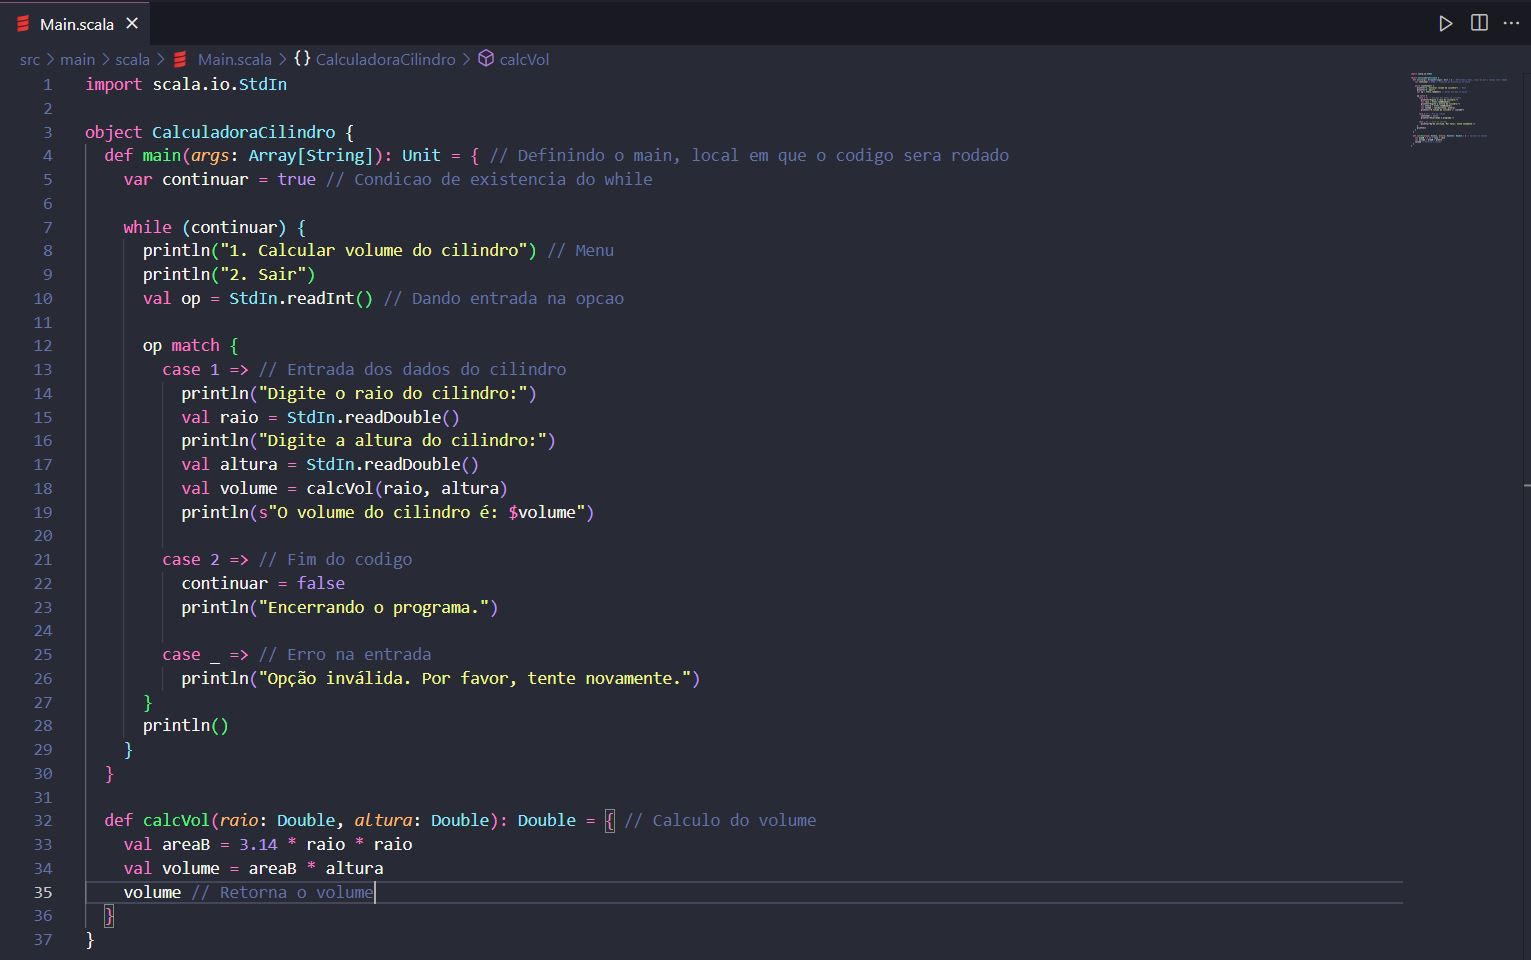
\includegraphics[width=17cm]{Pictures/Operac.jpg} \\
		Fonte: Autor do Livro
	\end{figure}

	Resultados ao compilar o arquivo:
	
	\begin{figure}[H]
		\centering
		\caption{Resultados Implementação Operações}
		\label{Resultados Implementação Operações}
		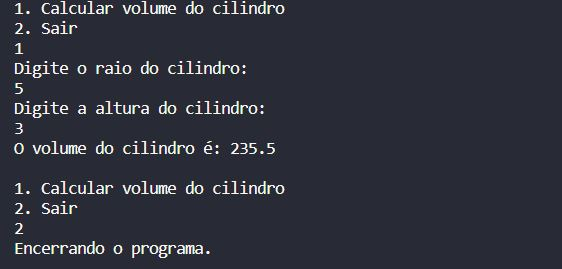
\includegraphics[width=8cm]{Pictures/ResOperac.jpg} \\
		Fonte: Autor do Livro
	\end{figure}


    %%%--------------------------------------------------------------------
    \section{Calculadora}
    %%%--------------------------------------------------------------------
    
   	O algoritmo a ser apresentado nesta seção é um exemplo simples de uma calculadora que é capaz de realizar as 4 operações matemáticas básicas: adição, subtração, multiplicação e divisão. O objetivo desse algoritmo é dar a possibilidade ao usuário de realizar as 4 operações com os números fornecidos.  
    
    Código fonte: 
    \begin{lstlisting}[breaklines]
// Definindo a classe Calculadora
class Calculadora {
	// Definindo as operacoes basicas da classe (metodos)
	def add(a: Int, b: Int): Int = a + b
	
	def sub(a: Int, b: Int): Int = a - b
	
	def mult(a: Int, b: Int): Int = a * b
	
	def div(a: Float, b: Float): Float = {
		if (b != 0) //Verificando se ocorre uma divisao por 0
		a / b
		else
		throw new ArithmeticException("Divisao por zero nao e permitida!")
	}
}

// Definindo o main, onde o programa sera rodado
object Main {
	def main(args: Array[String]): Unit = {
		// Criando uma instancia da classe Calculadora
		val calculadora = new Calculadora()
		
		// Realizando as operacoes
		val sum = calculadora.add(4, 2)
		val dif = calculadora.sub(4, 2)
		val prod = calculadora.mult(4, 2)
		val quot = calculadora.div(4, 2)
		
		// Imprimindo os resultados
		println(s"Soma: $sum")
		println(s"Diferenca: $dif")
		println(s"Produto: $prod")
		println(s"Quociente: $quot")
	}
}
    \end{lstlisting}
	\begin{itemize}
		\item Inicialmente, é definida uma classe chamada "calculadora", com seus 4 métodos que representam as 4 operações básicas.
		
		\item O método "add" recebe 2 valores inteiros e os soma, o método "sub" recebe 2 inteiros e os subtrai, o método "mult" recebe 2 inteiros e os multiplica, e por último o método "div" recebe 2 floats, verifica se o segundo é diferente de 0 (para evitar uma indefinição) e caso não seja será realizada a divisão de a por b.
		
		\item Em seguida é criado o main, local que será o ponto de partida do programa.
		
		\item No interior do main é criada uma nova instância da classe calculadora.
		
		\item Por meio dessa instância criada, são realizadas as operações matemáticas desejadas, armazenando os resultados em variáveis.
		
		\item E por último são mostrados os valores para o usuário.
	\end{itemize}

	A implementação desse código fonte em uma Ide é extremamente simples, basta criar um projeto e escrever o código em na Ide desejada. Neste caso, foi utilizado como Ide o Vscode, veja o exemplo abaixo:
	
	\begin{figure}[H]
		\centering
		\caption{Implementação Calculadora}
		\label{Implementação Calculadora}
		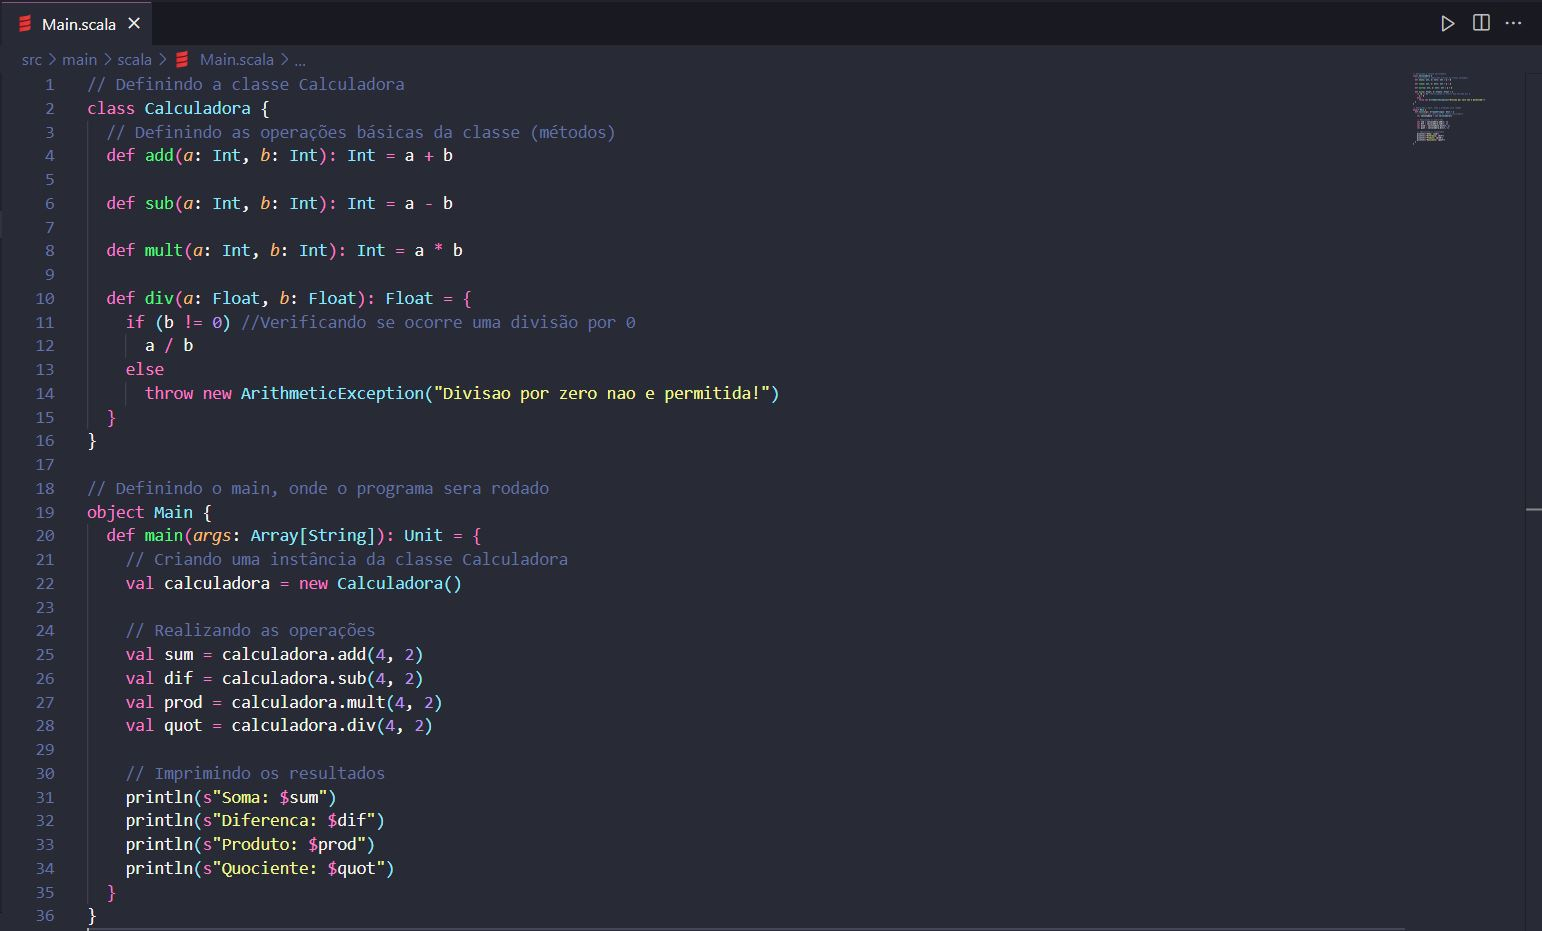
\includegraphics[width=17cm]{Pictures/Calc.jpg} \\
		Fonte: Autor do Livro
	\end{figure}

	Resultados obtidos ao compilar o algoritmo: 
	
	\begin{figure}[H]
		\centering
		\caption{Resultados Implementação Calculadora}
		\label{Resultados Implementação Calculadora}
		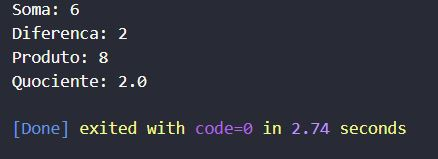
\includegraphics[width=8cm]{Pictures/ResCalc.jpg} \\
		Fonte: Autor do Livro
	\end{figure}
    %%%--------------------------------------------------------------------
    
    \section{Regra do Trapézio}
    Nessa seção será apresentada uma aplicação de um código em Scala responsável por calcular o valor aproximado de uma integral definida em um intervalo de a até b. Para isso será utilizado um conceito do cálculo numérico denominado Regra do Trapézio Generalizado.
    
    Código fonte:
    
    \begin{lstlisting}[breaklines]
object RegraDoTrapezio {
	def main(args: Array[String]): Unit = {
		val a = 0.0 // Limite inferior do intervalo
		val b = 2.0 // Limite superior do intervalo
		val n = 10 // Numero de subintervalos
		
		val h = (b - a) / n // Tamanho de cada subintervalo
		val x = Array.tabulate(n + 1)(i => a + i * h) // Pontos xi tal que i = 0, 1, ..., n
		val y = x.map(f) // Valores de f(xi) para cada xi
		
		val integral = (h / 2) * (y.head + 2 * y.drop(1).dropRight(1).sum + y.last)
		
		println(s"Aproximacao da integral: $integral")
	}
	
	def f(x: Double): Double = {
		// Definindo a funcao que sera integrada
		x * x // f(x) = x^2
	}
}
    \end{lstlisting} 

	\begin{itemize}
		\item Inicialmente no main é definido os limites inferiores e superiores da integral, assim o número de subintervalos que serão utilizados para o calculo.
		
		\item Com isso será calculado o valor de h, que será o passo entre os pontos de amostragem.
		
		\item Após calcular o h (o passo), será efetuado do valor de todos os xi relacionados a cada subintervalo, assim como o f(xi) associado a cada subintervalo.
		
		\item Com isso será calculado o valor aproximado da integral, para isso basta aplicar a formula da regra do trapézio generalizado:
		\[
		\text{{Integral}} \approx \frac{h}{2} \left( y_0 + 2 \sum_{i=1}^{n-1} y_i + y_n \right)
		\]
		onde:
		\begin{align*}
			h & : \text{{tamanho do subintervalo}} \\
			y_0, y_1, ..., y_n & : \text{{valores da função nos pontos de amostragem}}
		\end{align*}
	\end{itemize}
    
    Com isso já é possível implementar esse código em um ambiente de programação adequado. Para isso foi escolhido a Ide Vscode, veja abaixo a implementação do algoritmo e o valor obtido com sua compilação.
    
    Implementação:
    
	\begin{figure}[H]
		\centering
		\caption{Implementação Regra do Trapézio Generalizado}
		\label{Implementação Regra do Trapézio Generalizado}
		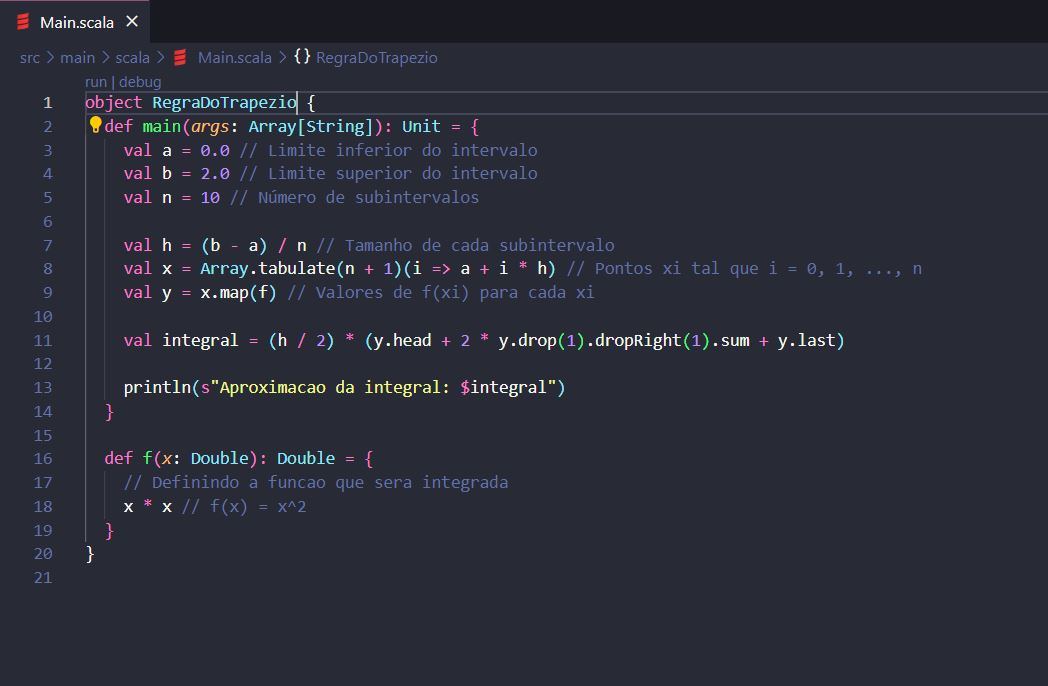
\includegraphics[width=17cm]{Pictures/Integral.jpg} \\
		Fonte: Autor do Livro
	\end{figure}
    
    Resultado obtido ao compilar o algoritmo: 
    
    \begin{figure}[H]
    	\centering
    	\caption{Resultados Implementação Regra do Trapézio Generalizado}
    	\label{Resultados Implementação Regra do Trapézio Generalizado}
    	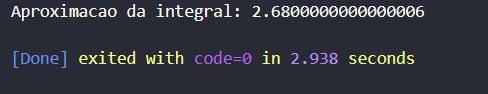
\includegraphics[width=8cm]{Pictures/ResIntegral.jpg} \\
    	Fonte: Autor do Livro
    \end{figure}
    
    \section{Bubble Sort}
    %%%--------------------------------------------------------------------
    O bubble sort é um clássico algoritmo de ordenação de dados muito utilizado para organizar valores de um vetor. O algoritmo funciona percorrendo todos os elementos de uma lista, comparando os valores adjacentes e caso estejam na ordem errada é realizada uma troca. Isso ocorre até o array estar completamente ordenado.
      
    Código fonte:
    \begin{lstlisting}[breaklines]
object BubbleSortExample {
	def BubbleSort(arr: Array[Int]): Array[Int] = { // Funcao de bubble sort
		val n = arr.length // Definindo o tamanho do array
		for (i <- 0 until n - 1) { // For para percorrer o array
			for (j <- 0 until n - i - 1) { // For para percorrer o array e realizar as comparacoes
				if (arr(j) > arr(j + 1)) { // Verificando se o proximo valor e menor que o valor atual
					val temp = arr(j) // Troca
					arr(j) = arr(j + 1)
					arr(j + 1) = temp
				}
			}
		}
		arr // Retorna
	}
	
	def main(args: Array[String]): Unit = { // Definindo o main
		val array = Array(64, 34, 25, 12, 22, 11, 90) // Definindo o array
		val sortArray = BubbleSort(array) // Chamada da funcao
		println(sortArray.mkString(", ")) // Mostrando para o usuario
	}
}
    \end{lstlisting}

	\begin{itemize}
		\item Inicialmente no main, é definido um array com elementos aleatórios de maneira desordenada.
		
		\item Em seguida é realizada a chamada da função bubble sort.
		
		\item Logo em seguida, o tamanho do array é salvo na variável.
		
		\item Em seguida é criado um for externo responsável por percorrer o array.
		
		\item Também é criado um for interno, responsável por percorrer o array e realizar as comparações entre o elemento na posição j e seu sucessor, caso o valor na posição j seja maior que na posição j + 1, ocorre uma troca.
		
		\item Com o fim de ambos os loops, o array organizado é retornado e mostrado ao usuário.
	\end{itemize}

	A implementação desse algoritmo, assim como as anteriores, foi feita criando um projeto na Ide Vscode, veja abaixo a implementação e o resultado obtido com a compilação do arquivo.
	
	Implementação:

	\begin{figure}[H]
		\centering
		\caption{Implementação Bubble Sort}
		\label{Implementação Bubble Sort}
		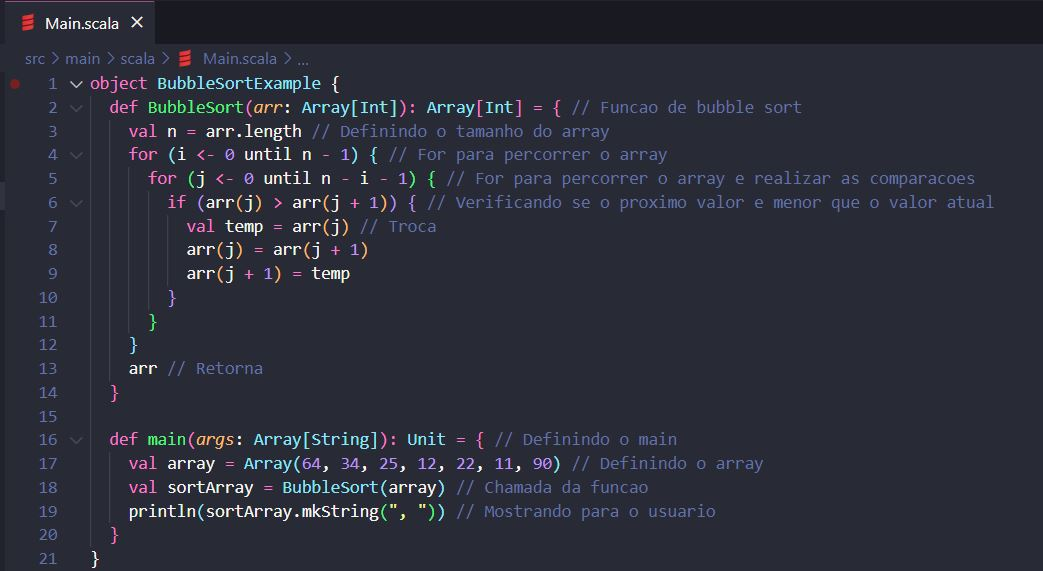
\includegraphics[width=17cm]{Pictures/bubble.jpg} \\
		Fonte: \href{https://www.includehelp.com/scala/implement-an-arithmetic-calculator-using-a-match-case.aspx}{Clique Aqui}
	\end{figure}

	Resultados obtidos quando o arquivo é compilado:

	\begin{figure}[H]
		\centering
		\caption{Resultados Implementação Bubble Sort}
		\label{Resultados Implementação Bubble Sort}
		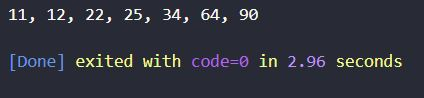
\includegraphics[width=8cm]{Pictures/resBubble.jpg} \\
		Fonte: \href{https://www.includehelp.com/scala/implement-an-arithmetic-calculator-using-a-match-case.aspx}{Clique Aqui}
	\end{figure}

    %%%--------------------------------------------------------------------
    \section{Quick Sort}
    %%%--------------------------------------------------------------------
    O quick sort é um clássico e extremamente efetivo algoritmo de ordenação, por isso recebe o nome de quick sort. Ele funciona selecionando um elemento do array que será chamado de pivô, com isso é seguido a lógica de separar o vetor em 2, uma parte com valores menores que o pivô e outra parte com valores maiores que o pivô, buscando assim coloca-lo em sua respectiva posição.
    
    Código fonte:
    
    \begin{lstlisting}[breaklines]
object QuickSort {
	def main(args: Array[String]): Unit = { // Main
		val arr = Array(64, 34, 25, 12, 22, 11, 90) // Definindo array
		println("Array antes da ordenacao:")
		println(arr.mkString(", "))
		
		quickSort(arr, 0, arr.length - 1) // Chamada da funcao
		
		println("Array apos a ordenacao:")
		println(arr.mkString(", "))
	}
	
	def quickSort(arr: Array[Int], a: Int, b: Int): Unit = { // Definindo funcao quick sort
		if (a < b) { // Caso ainda tenham dados no array
			val pivo = partition(arr, a, b)
			
			// Chamadas recursivas
			quickSort(arr, a, pivo - 1)
			quickSort(arr, pivo + 1, b)
		}
	}
	
	def partition(arr: Array[Int], a: Int, b: Int): Int = {
		val pivo = arr(b) // Define o pivo
		var i = a - 1 
		
		for (j <- a until b) { // Loop para percorrer o array
			if (arr(j) <= pivo) { // Procurando menor valor
				i += 1
				swap(arr, i, j) // Funcao de troca
			}
		}
		
		swap(arr, i + 1, b) // Funcao de troca
		i + 1
	}
	
	def swap(arr: Array[Int], i: Int, j: Int): Unit = { // Funcao de troca
		val temp = arr(i)
		arr(i) = arr(j)
		arr(j) = temp
	}
}
    \end{lstlisting}

	\begin{itemize}
		\item Inicialmente é criado o main e dentro dele é também criado o array com valores aleatórios de maneira desordenada, em seguida é realizada a chamada da função, passando como parâmetros o próprio array, o início e o fim.
		
		\item Após isso é verificado se ainda existem elementos no vetor, se verdadeiro é chamada a função que repartira o array e selecionará o pivô.
		
		\item Dentro dessa função é definido o pivô como o último elemento do array, dentro do loop é verificado se o elemento for menor ou igual ao pivô, incrementamos i e trocamos o elemento na posição i com o elemento na posição j.
		
		\item Após o loop, o último elemento menor ou igual ao pivô está na posição i + 1. Portanto, trocamos o pivô de posição com esse elemento para colocá-lo em sua posição final.
		
		\item Com o fim do loop é retornado a posição do pivô, com isso são feitas as chamadas recursivas dividindo novamente o array, sendo a primeira chamada feita para organizar a esquerda a lista, e a segunda para ordenar a direita do array.
	\end{itemize}

	A implementação desse algoritmo, assim como as anteriores, foi feita criando um projeto na Ide Vscode, veja abaixo a implementação e o resultado obtido com a compilação do arquivo.
	
	Implementação:
	
	\begin{figure}[H]
		\centering
		\caption{Implementação Quick Sort Parte 1}
		\label{Implementação Quick Sort Parte 1}
		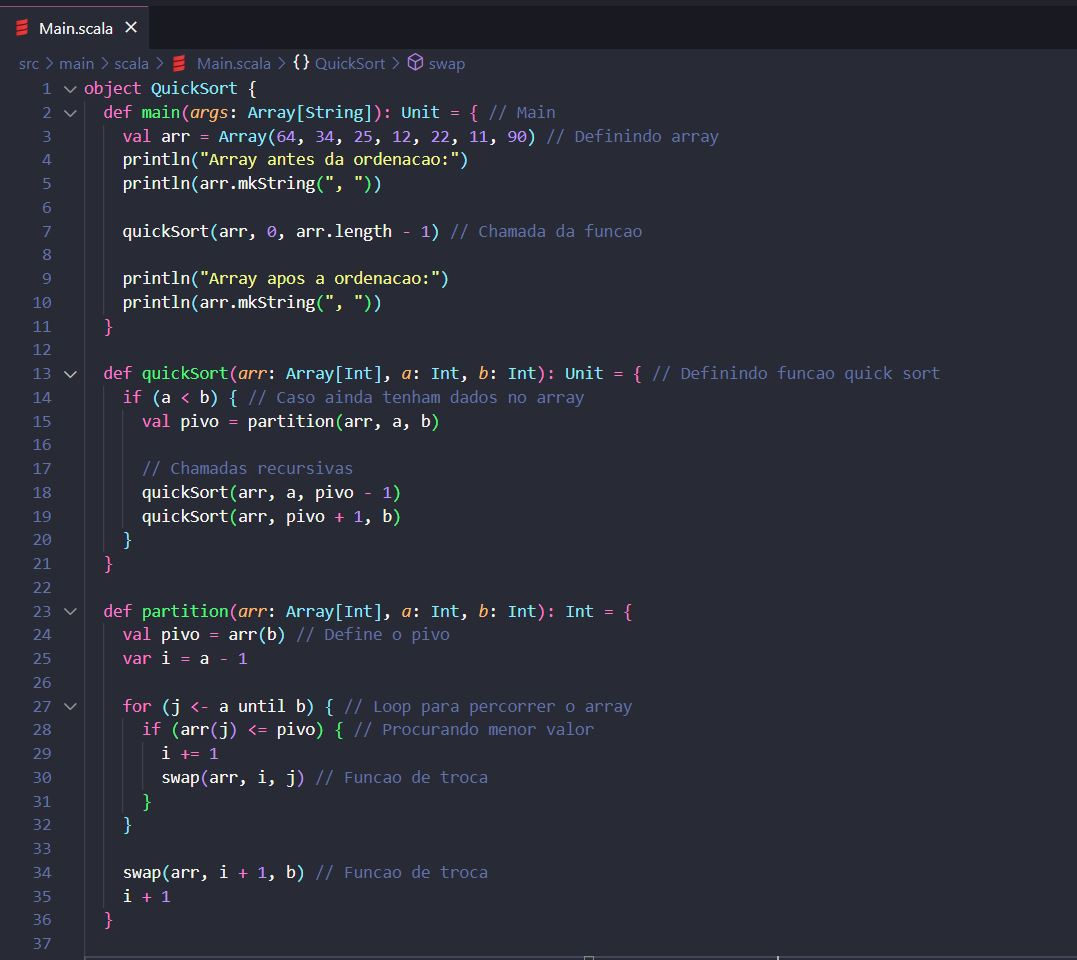
\includegraphics[width=17cm]{Pictures/Quick1.jpg} \\
		Fonte: \href{https://stackoverflow.com/questions/67182087/scala-quicksort-algorithm-implementationi}{Clique Aqui!}
	\end{figure}

	 \begin{figure}[H]
	 	\centering
	 	\caption{Implementação Quick Sort Parte 2}
	 	\label{Implementação Quick Sort Parte 2}
	 	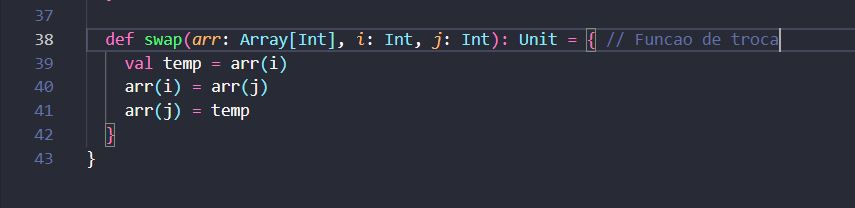
\includegraphics[width=12cm]{Pictures/Quick2.jpg} \\
	 	Fonte: \href{https://stackoverflow.com/questions/67182087/scala-quicksort-algorithm-implementationi}{Clique Aqui!}
	 \end{figure}
 
 	Resultados obtidos ao compilar:
 
 	\begin{figure}[H]
	 	\centering
	 	\caption{Resultados Implementação Quick Sort}
	 	\label{Resultados Implementação Quick Sort}
	 	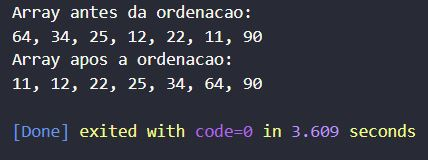
\includegraphics[width=8cm]{Pictures/resQuick.jpg} \\
	 	Fonte: \href{https://stackoverflow.com/questions/67182087/scala-quicksort-algorithm-implementationi}{Clique Aqui!}
 	\end{figure}
 	
 	\section{Equação do Segundo Grau}
 	
 	Essa seção abordará um algoritmo básico de cálculo de uma equação do segundo grau utilizando a conhecida fórmula de bhaskhara. O objetivo desse algoritmo é encontrar as raízes de uma equação do segundo grau fornecida ao programa.
 	
 	\begin{lstlisting}[breaklines]
import scala.math.sqrt // Biblioteca para calculo de raiz

object EquacaoSegundoGrau {
	def CalcEq(a: Double, b: Double, c: Double): Unit = { 
		val delta = b * b - 4 * a * c // Calculo delta
		
		if (delta > 0) { // Existem 2 raizes reais
			val x1 = (-b + sqrt(delta)) / (2 * a) // Calculo raiz 1
			val x2 = (-b - sqrt(delta)) / (2 * a) // Calculo raiz 2
			println("Raizes:")
			println(s"x1 = $x1")
			println(s"x2 = $x2")
		} else if (delta == 0) { // Existe 1 raiz
			val x = -b / (2 * a) // Calculo da raiz
			println("Raiz:")
			println(s"x = $x")
		} else {
			println("A equacao nao possui raizes reais.") // Delta < 0, logo raiz imaginaria
		}
	}
	
	def main(args: Array[String]): Unit = { // Main
		// Coeficientes equacao
		val a = 1.0
		val b = -3.0
		val c = 2.0
		
		CalcEq(a, b, c) // Chamada funcao
	}
}
 	\end{lstlisting}  
 
 	\begin{itemize}
 		\item Inicialmente é dado o import na biblioteca responsável por calcular o valor da raiz quadrada.
 		
 		\item no main é dada a entrada dos coeficientes da equação do segundo grau.
 		
 		\item Na função chamada, é calculado inicialmente o delta, em seguida é verificado se o mesmo é maior que 0, se sim existem 2 raízes que serão calculada e retornadas, se for zero existe apenas uma raiz, e se for menor que 0 ocorrerá uma raiz quadrada de número negativo, logo uma raiz imaginária.
 		
 		\item Em seguida o valor é mostrado ao usuário.
 	\end{itemize}
 
 	A implementação desse código fonte em uma Ide é extremamente simples, basta criar um projeto e escrever o código em na Ide desejada. Neste caso, foi utilizado como Ide o Vscode, veja o exemplo abaixo:
 	
 	Implementação:
 	
 	\begin{figure}[H]
 		\centering
 		\caption{Implementação Equação 2 Grau}
 		\label{Implementação Equação 2 Grau}
 		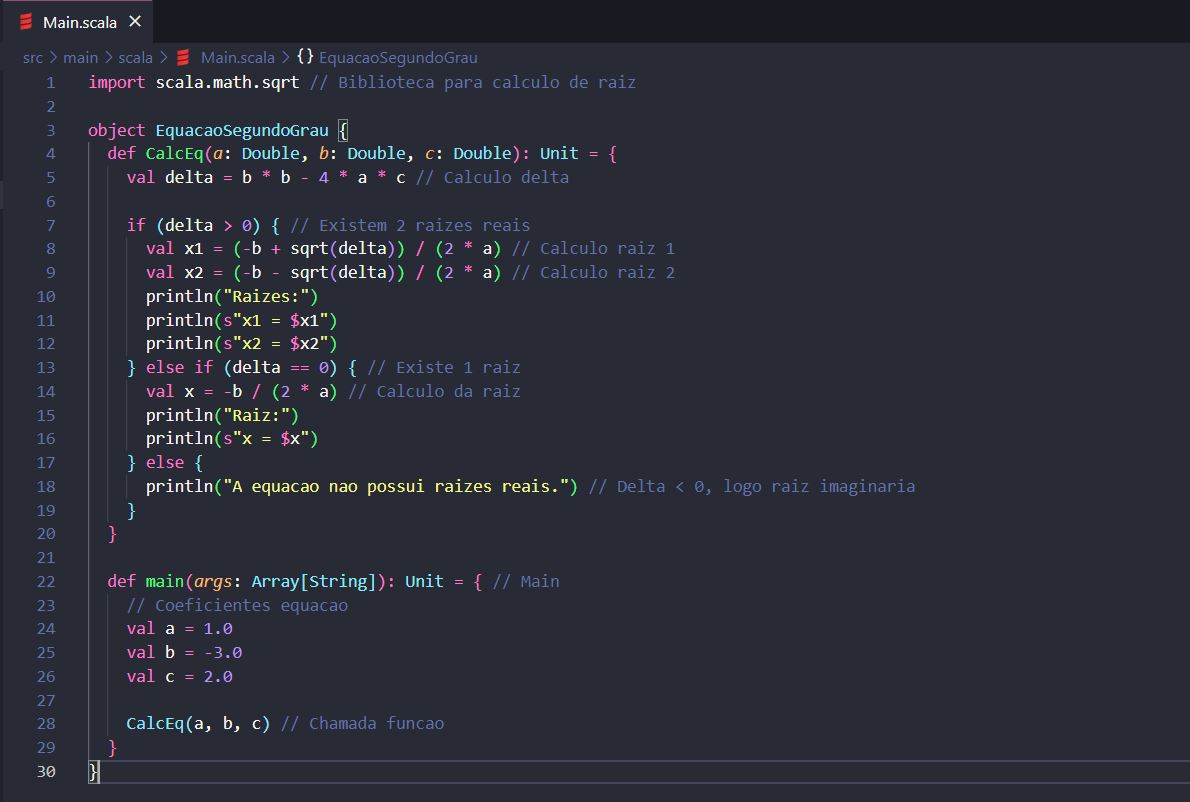
\includegraphics[width=17cm]{Pictures/Eq2Grau.jpg} \\
 		Fonte: Autor do Livro
 	\end{figure}
 	
 	Resultados da compilação:
 	
 	\begin{figure}[H]
		\centering
		\caption{Resultados Equação do 2 Grau}
		\label{Resultados Equação do 2 Grau}
		\includegraphics[width=8cm]{Pictures/resEq2Grau.jpg} \\
		Fonte: Autor do Livro
	\end{figure}


	\section{Sistema Linear}
	
	Nesta seção abordaremos um algoritmo capaz de solucionar um sistema de equações 2x2. Para isso é necessário calcular o determinante da matriz com o objetivo de verificar se existe solução, e caso esse determinante seja diferente de 0, será efetuada a regra de cramer para calcular a solução do sistema.
	
	Código fonte: 
	
	\begin{lstlisting}[breaklines]
object SistemaEquacoes {
	
	def resSist(a11: Double, a12: Double, b1: Double, a21: Double, a22: Double, b2: Double): Option[(Double, Double)] = {
		val det = a11 * a22 - a12 * a21 // Calculo do determinante
		
		if (det != 0) {
			// Calculo solucao
			val x = (b1 * a22 - b2 * a12) / det
			val y = (a11 * b2 - a21 * b1) / det
			Some(x, y)
		} else {
			None // O sistema nao tem solucao unica
		}
	}
	
	def main(args: Array[String]): Unit = {
		// Coeficientes
		val a11 = 2.0
		val a12 = 3.0
		val b1 = 10.0
		val a21 = 1.0
		val a22 = -1.0
		val b2 = -5.0
		
		val solucao = resSist(a11, a12, b1, a21, a22, b2) // Chamada funcao
		
		solucao match {
			case Some((x, y)) =>
			println(s"Solucao: x = $x, y = $y")
			case None =>
			println("O sistema nao tem solucao unica...")
		}
	}
	
}
	\end{lstlisting}

 	\begin{itemize}
 		\item Inicialmente no main é se define o sistema linear desejado no seguinte formato:
 		\begin{lstlisting}
		a11 * x + a12 * y = b1
		a21 * x + a22 * y = b2
 		\end{lstlisting}
 		Com isso é realizada a chamada da função que irá calcular a solução.
 		\item Na função de cálculo de solução é inicialmente calculado o determinante, para verificar se o sistema em questão possui solução ou não, caso o determinante seja diferente de zero é realizada a regra de cramer que dará como resultado a solução do sistema, retornando assim para o usuário. Porém caso o determinante seja igual a 0 será retornado 'none', indicando que o sistema não possui solução única.
 	\end{itemize}
 
 	 Com isso já é possível implementar esse código em um ambiente de programação adequado. Para isso foi escolhido a Ide Vscode, veja abaixo a implementação do algoritmo e o valor obtido com sua compilação.
 	 
 	 Implementação:
 	 
 	 \begin{figure}[H]
 	 	\centering
 	 	\caption{Implementação Sistema Linear}
 	 	\label{Implementação Sistema Linear}
 	 	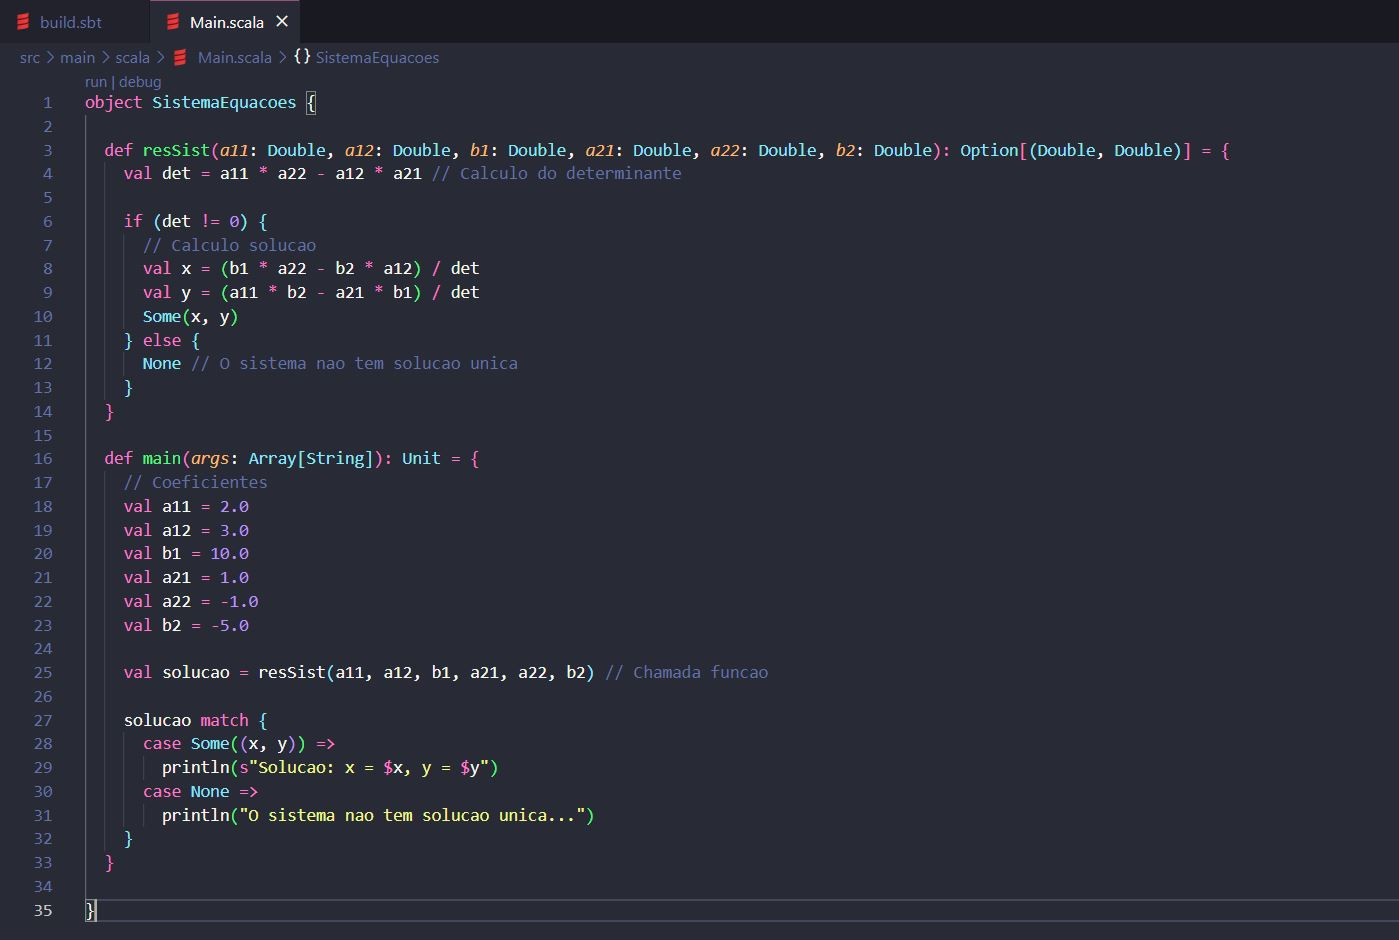
\includegraphics[width=17cm]{Pictures/Sist.jpg} \\
 	 	Fonte: Autor do Livro
 	 \end{figure}
  
  
	 Resultados da compilação:
	  
	\begin{figure}[H]
	 	\centering
	 	\caption{Resultados Sistema Linear}
	 	\label{Resultados Sistema Linear}
	 	\includegraphics[width=8cm]{Pictures/resSist.jpg} \\
	 	Fonte: Autor do Livro
	\end{figure}
